\section{Evaluation}

To systematically evaluate \SysName, we structure our experiments around the following research questions:
% \begin{itemize}[leftmargin=*]
%     \vspace{-0.65em}
%     \item \textbf{RQ1:} What end-to-end throughput improvement does \SysName achieve for offline large-batch agentic inference? (\S\ref{subsec:evalrq1})
    
%     \item \textbf{RQ2:} How does \SysName influence KV cache behavior under high concurrency, in terms of cache hit rate and memory utilization? (\S\ref{subsec:evalrq2})
    
%     \item \textbf{RQ3:} Can a fixed-size admission control policy adequately support agentic workloads? (\S\ref{subsec:evalrq3})

% \end{itemize}

\noindent \textbf{Q1:} What end-to-end throughput improvement does \SysName achieve for offline batch agentic inference? (\S\ref{subsec:evalrq1})

\noindent \textbf{Q2:} How does \SysName influence KV cache behavior under high concurrency, in terms of cache hit rate and memory utilization? (\S\ref{subsec:evalrq2})

\noindent \textbf{Q3:} Can a fixed-size admission control policy adequately support agentic workloads? (\S\ref{subsec:evalrq3})


% \noindent\textbf{Testbed.}


% \noindent\textbf{Models and Algorithms.}
% We conduct a thorough evaluation on Qwen3-32B and DeepSeekV3.1 model with real-world BrowserComputer \cite{browsecomp} datasets.

% \noindent\textbf{Metrics.}
% We measure inference efficiency via end-to-end wall-clock latency. 

% \begin{figure*}[tb]
%     \centering
% \includegraphics[width=0.98\linewidth]{figure/e2e_speedup_comparison.pdf
% }
%     \caption{End-to-end latency of offline agentic inference under increasing effective concurrency.
% The x-axis labels denote configurations of \emph{batch size/tensor parallelism degree/number of GPUs}, respectively.}
%     \label{fig:e2ecomparisons}
%     % \vvspace{}
% \end{figure*}

\begin{table*}[t]
\caption{End-to-end latency and Speedup of offline agentic inference under increasing effective concurrency, reported in seconds. }
\centering
\small
\begin{tabular}{l l c c c c}
\toprule
\textbf{Model} & \textbf{Batch / TP / \#GPU} 
& \textbf{SGLang (s)} 
& \textbf{SGLang w/ Request Control (s)} 
& \textbf{SGLang w/ HiCache (s)} 
& \textbf{\SysName} (s)\\
\midrule


& 256 / 8 / 8
& 1480 (1.00$\times$)
& 2049 (0.72$\times$)
& 976 (1.52$\times$)
& \textbf{362 (4.09$\times$)} \\

Qwen3-32B & 256 / 4 / 4
& 2213 (1.00$\times$)
& 1089 (2.03$\times$)
& 1678 (1.32$\times$)
& \textbf{757 (2.92$\times$)} \\

& 256 / 2 /2
& 2527 (1.00$\times$)
& 1383 (1.83$\times$)
& 1112 (2.27$\times$)
& \textbf{846 (2.99$\times$)} \\

\midrule
& 16 / 16 / 16
& 873 (1.00$\times$)
& 861 (1.01$\times$)
& 2559 (0.34$\times$)
& \textbf{521 (1.68$\times$)} \\

DeepSeek-V3
& 32 / 16 / 16
& 1226 (1.00$\times$)
& 1367 (0.90$\times$)
& 2277 (0.54$\times$)
& \textbf{1018 (1.20$\times$)} \\

& 40 / 16 / 16
& 3877 (1.00$\times$)
& 2903 (1.34$\times$)
& 2320 (1.67$\times$)
& \textbf{2043 (1.90$\times$)} \\

\bottomrule
\end{tabular}

\label{tab:end_to_end_latency}
\end{table*}


\begin{table}[t]
\caption{KV Cache Hit Rate (\%) under varying batch sizes and concurrency levels for DeepSeek-V3 with TP=8 on 8 GPUs. \SysName maintains higher hit rates compared to baselines.}
\centering
\footnotesize
\label{tab:kv_hit_rate}
% \begin{tabular}{c c c c c}
\begin{tabular}{>{\centering\arraybackslash}p{0.8cm} 
                >{\centering\arraybackslash}p{1.2cm} 
                >{\centering\arraybackslash}p{1.5cm} 
                >{\centering\arraybackslash}p{1.8cm} 
                >{\centering\arraybackslash}p{1.2cm}}
\toprule
Batch  & SGLang (\%) & SGLang w/ HiCache (\%) & SGLang w/ Request Control (\%) & \SysName (\%) \\
\midrule
16 & 80.38 & 97.48 & 69.00 & 96.38 \\
32 & 77.72 & 97.13 & 68.39 & 93.65 \\
40  & 35.41 & 96.08 & 32.21 & 73.36 \\
\bottomrule
\end{tabular}
\end{table}







\subsection{End-to-End Performance}
\label{subsec:evalrq1}
% RQ1
To answer Q1, we evaluate the end-to-end latency of offline batch agentic inference under varying concurrency levels.
We compare \SysName with three baselines:
(i) \textbf{SGLang}, which relies on request-level batching with LRU-based KV cache eviction;
(ii) \textbf{SGLang with request-level admission control}, which limits concurrency using a fixed request-level cap;
and (iii) \textbf{SGLang with HiCache}, a cache-centric approach that prioritizes KV cache retention and CPU offloading.
%and (iv) \textbf{Cache-Aware Admission Control} (\SysName), which regulates execution at agent granularity using dynamic admission control.
All systems use identical model weights, prompts, and rollout workloads. All experiments are conducted on NVIDIA H100 GPUs (80GB) interconnected with 900 GB/s NVLink, and connected across nodes via 8× 400 Gbps RoCE. The software stack includes PyTorch 2.7.1, Python 3.12, and CUDA 12.6.

\noindent\textbf{Hyperparameter Configuration.}
In our implementation, we fix all control parameters across experiments.
Following well-established best practices in AIMD-based congestion control, we set the additive increase factor to $\alpha = 2$ and the multiplicative decrease factor to $\beta = 0.5$, which strike a standard balance between stable capacity probing and rapid recovery under congestion. 
The utilization and cache-hit thresholds are configured as $U_{low} = 0.2$, $U_{high} = 0.5$, and $H_{thresh} = 0.2$. 
We conduct a sensitivity analysis on the utilization thresholds in Appendix~\ref{appendix:sensitivity}. 
The results show that $U_{high}$ can be selected from a relatively broad, non-sensitive operating range (0.5--0.6), while $U_{low}$ requires more careful calibration as it directly controls the aggressiveness of window increases. Our choice of $U_{low} = 0.2$ and $U_{high} = 0.5$ balances proactive capacity exploration with timely congestion response.
All parameters are kept constant for all models, workloads, and serving engines.




We report the end-to-end batch latency for two representative large models, Qwen3-32B and DeepSeek-V3, under increasing effective concurrency controlled via batch size and tensor parallelism (TP). Lower latency indicates higher effective throughput for offline agentic inference. Table \ref{tab:end_to_end_latency} presents the end-to-end latency across all configurations.
\SysName consistently achieves the lowest latency across both models and all concurrency settings, with particularly large gains under high-concurrency regimes. For Qwen3-32B, \SysName reduces latency by up to $4.09\times$ compared to SGLang and $2.8\times$ compared to request-level admission.
The performance gap widens as TP decreases and effective per-GPU concurrency increases, where baseline systems experience severe slowdowns.
Similarly, for DeepSeek-V3, \SysName outperforms all baselines under large batch sizes, avoiding the drastic latency inflation observed in SGLang and cache-centric approaches.

The poor performance of request- and cache-centric baselines stems from their inability to align scheduling decisions with agent-level memory locality.
Request-level admission lacks visibility into the accumulated KV cache footprint of long-running agents, often delaying their execution until cached state has already been evicted, leading to repeated recomputation.
Cache-centric approaches (e.g., HiCache) reduce recomputation by offloading KV cache slots to CPU memory, but under high concurrency, PCIe contention and queueing delays dominate, limiting their effectiveness.

By contrast, \SysName regulates concurrency at the agent level, directly bounding the aggregate KV cache working set of active agents.
This prevents over-admission during the middle phase of execution, preserves high cache hit rates, and maintains stable batch efficiency throughout inference.
As a result, \SysName achieves consistently low latency across models and batch sizes, explaining its advantage over fixed-cap and cache-centric baselines.

\begin{figure}[tb]
    \centering
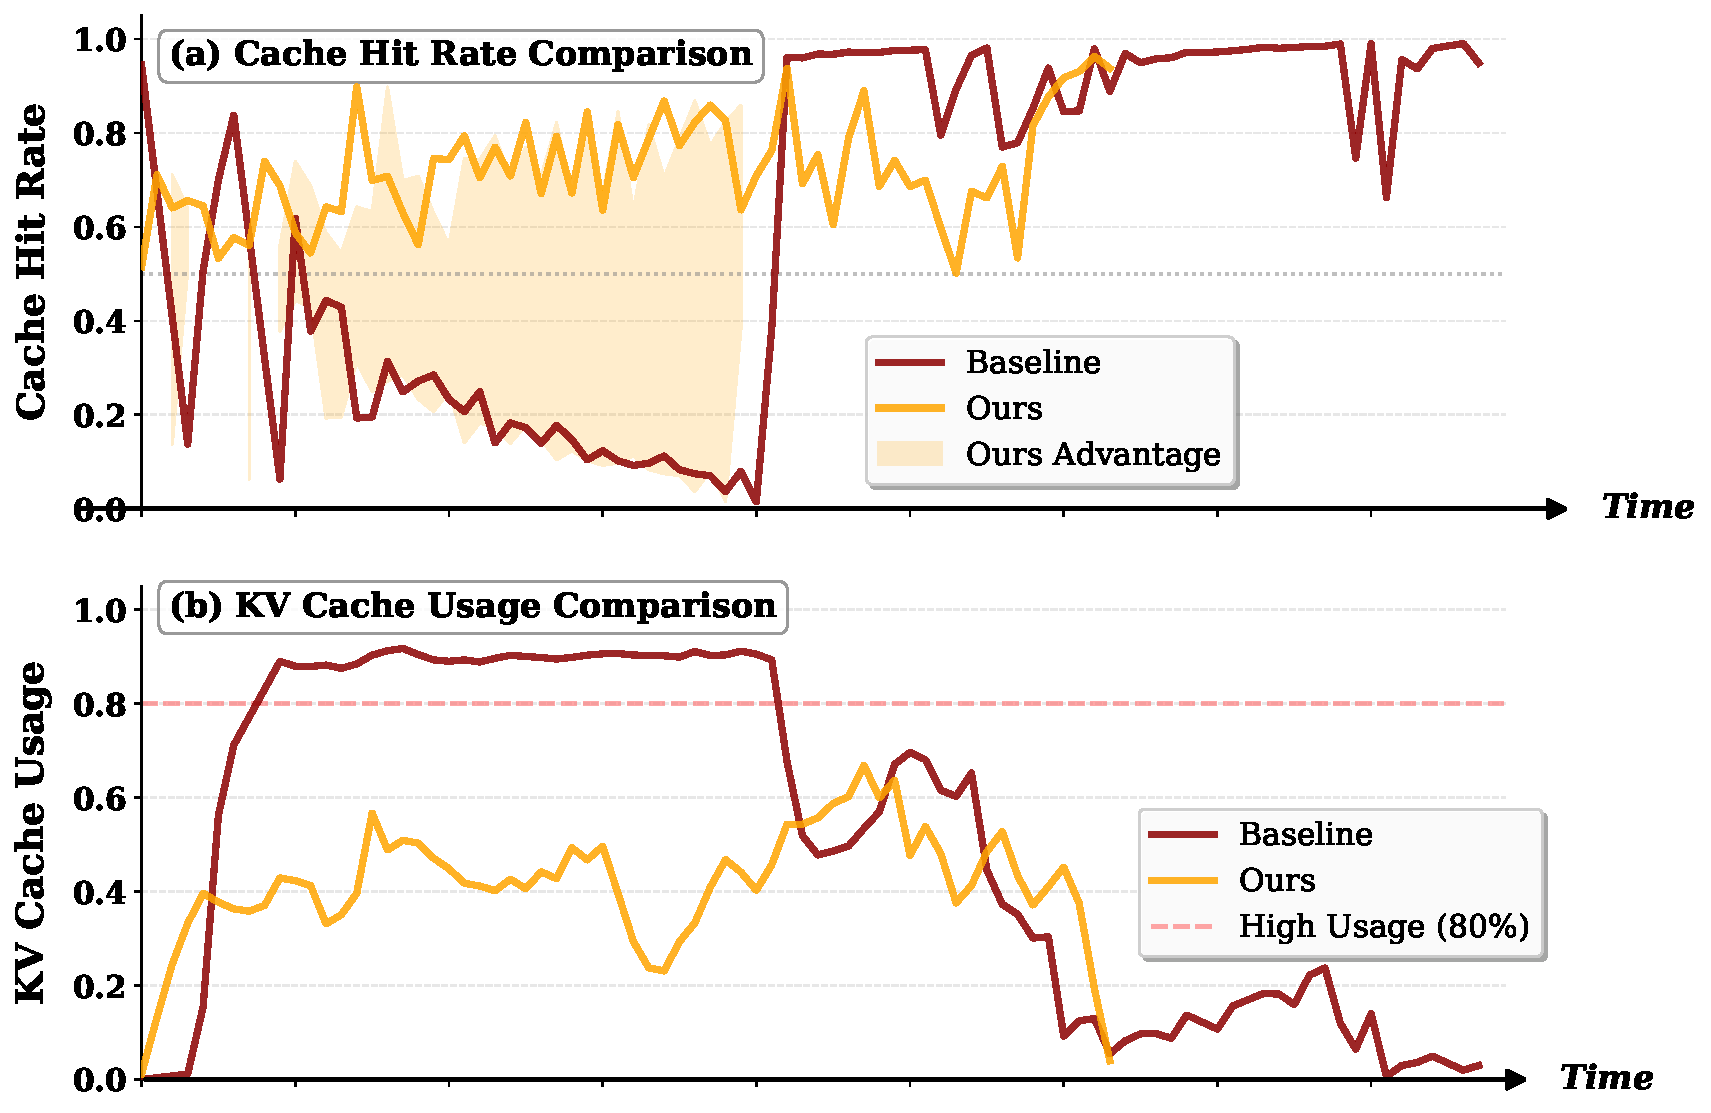
\includegraphics[width=0.98\linewidth]{figure/dual_kv_cache_comparison.pdf
}
    \caption{Temporal dynamics of KV cache during large-batch offline agentic inference for Qwen3-32B under constraint resources (Batch 256, TP=2, 2 GPUs).}
    \label{fig:kv_time_series}
    % \vvspace{}
\end{figure}

% SGLang's overcommitment triggers frequent KV cache evictions and recomputation. Although SGLang with request-level admission control limits the number of concurrent requests, it lacks visibility into agent-level execution state and KV cache footprint.
% As a result, a long-running agent with a large and valuable KV cache may be left waiting in the request queue while other requests (often with low KV cache hit rates due to prior eviction) are repeatedly scheduled. By the time the long agent is admitted, its KV cache has already been evicted, triggering expensive recomputation. This misalignment between scheduling decisions and agent-level memory locality leads to worse performance than both SGLang and agent-aware control. Cache-centric approaches (HiCache) mitigate recomputation by offloading KV tensors to CPU memory.
% However, under high concurrency, PCIe bandwidth contention and queueing delays dominate, resulting in limited performance gains and, in some cases, worse latency than recomputation-based baselines.

% \SysName avoids this pathological regime by regulating concurrency at the agent level.
% During the warmup phase, when agents have short contexts and low KV cache footprints, the controller admits a large number of agents to fully utilize GPU compute.
% As execution progresses and agents enter mid-horizon steps, the controller detects rising memory pressure through cache usage and hit-rate signals and proactively reduces the number of admitted agents.
% This prevents the aggregate working set from exceeding GPU memory capacity, preserving high KV cache hit rates and stable batch efficiency.
% Finally, during the cooldown phase, as agents complete execution, concurrency is gradually increased again to reclaim idle capacity. By preventing over-admission rather than reacting to its consequences, \SysName maintains low latency across all phases of agent execution.
% This adaptive behavior explains why \SysName consistently outperforms fixed-cap and cache-centric baselines in large-batch agentic inference.

% \paragraph{Takeaway.}
% These results demonstrate that naive concurrency scaling is counterproductive for offline agentic inference.
% Effective end-to-end performance requires phase-aware, agent-level admission control that explicitly accounts for the evolving KV cache working set.
% \SysName provides such control, enabling stable and scalable inference where existing serving architectures fail.




\subsection{KV Cache Behavior Analysis}
\label{subsec:evalrq2}
% RQ2

% \begin{figure}[tb]
%     \centering
% \includegraphics[width=0.98\linewidth]{figure/cache_usage_comparison.pdf
% }
%     \caption{Average KV Cache Usage of offline agentic inference under increasing effective concurrency.
% The x-axis labels denote configurations of \emph{batch size/tensor parallelism degree/number of GPUs}, respectively.}
%     \label{fig:e2ecache}
%     % \vvspace{}
% \end{figure}


Table \ref{tab:kv_hit_rate} reports the average KV cache hit rate under the same configurations as \S\ref{subsec:evalrq1} of DeepSeek-V3. The results strongly correlate with the end-to-end latency trends observed earlier and provide direct evidence of middle-phase thrashing.

SGLang exhibits a rapid degradation in KV cache hit rate as concurrency increases.
While hit rates remain moderately high at small batch sizes, they collapse to $35.41\%$ at the configuration of a large batch size of 40. Despite limiting the number of in-flight requests, the request-level admission control hit rate drops to $32.21\%$ under high concurrency. HiCache achieves consistently high hit rates across all settings by aggressively retaining KV cache through CPU offloading. However, as shown in \S\ref{subsec:evalrq1}, high hit rates alone are insufficient to guarantee low latency, since the latency overhead induced by PCIe transmission negates this advantage. 

In contrast, \SysName maintains high KV cache hit rates while avoiding excessive offloading.
By regulating concurrency at agent granularity, it preserves KV locality during the thrashing phase without overcommitting memory.
This balanced behavior explains why it achieves the lowest latency in Q1 while maintaining substantially higher hit rates than SGLang and request-level baselines.


To better understand the temporal dynamics, Figure~\ref{fig:kv_time_series} plots KV cache hit rate (top) and KV cache usage (bottom) over time for a batch size of 256 agentic inference. As multiple agents concurrently progress through mid-horizon steps, KV cache usage approaches capacity (about 80\%) while the hit rate for the baseline drops sharply. \SysName maintains a significantly higher hit rate by regulating agent admission, preventing simultaneous overcommitment of KV cache slots.

\subsection{Static vs Cache-aware Admission Control}
\label{subsec:evalrq3}
To answer Q3, we evaluate whether a fixed-size admission control policy is sufficient for agentic workloads. We test several fixed admission control levels (30, 32, 64, 128) and compare them against our adaptive policy (\SysName).

Figure \ref{fig:e2ecache} shows the results. Small fixed levels (e.g., 30–64) reduce latency compared to the uncontrolled baseline, but are conservative and underutilize GPU resources at certain execution phases. Larger levels (e.g., 128) allow more concurrency but cause memory overcommitment, leading to KV cache thrashing and increased latency. \SysName reveals the lowest observed latency of 846 ms, $1.5–2.9\times$ improvement over the best fixed-level configurations and $2.99\times$ improvement over the baseline.

To summarize, static admission control is a brittle approach: it either underutilizes GPU resources or triggers KV cache thrashing depending on the chosen level. In contrast, \SysName is essential to achieve both high throughput and stable execution for agentic workloads, providing a principled, phase-aware regulation of concurrency that cannot be achieved with fixed-size policies.

\begin{figure}[tb]
    \centering
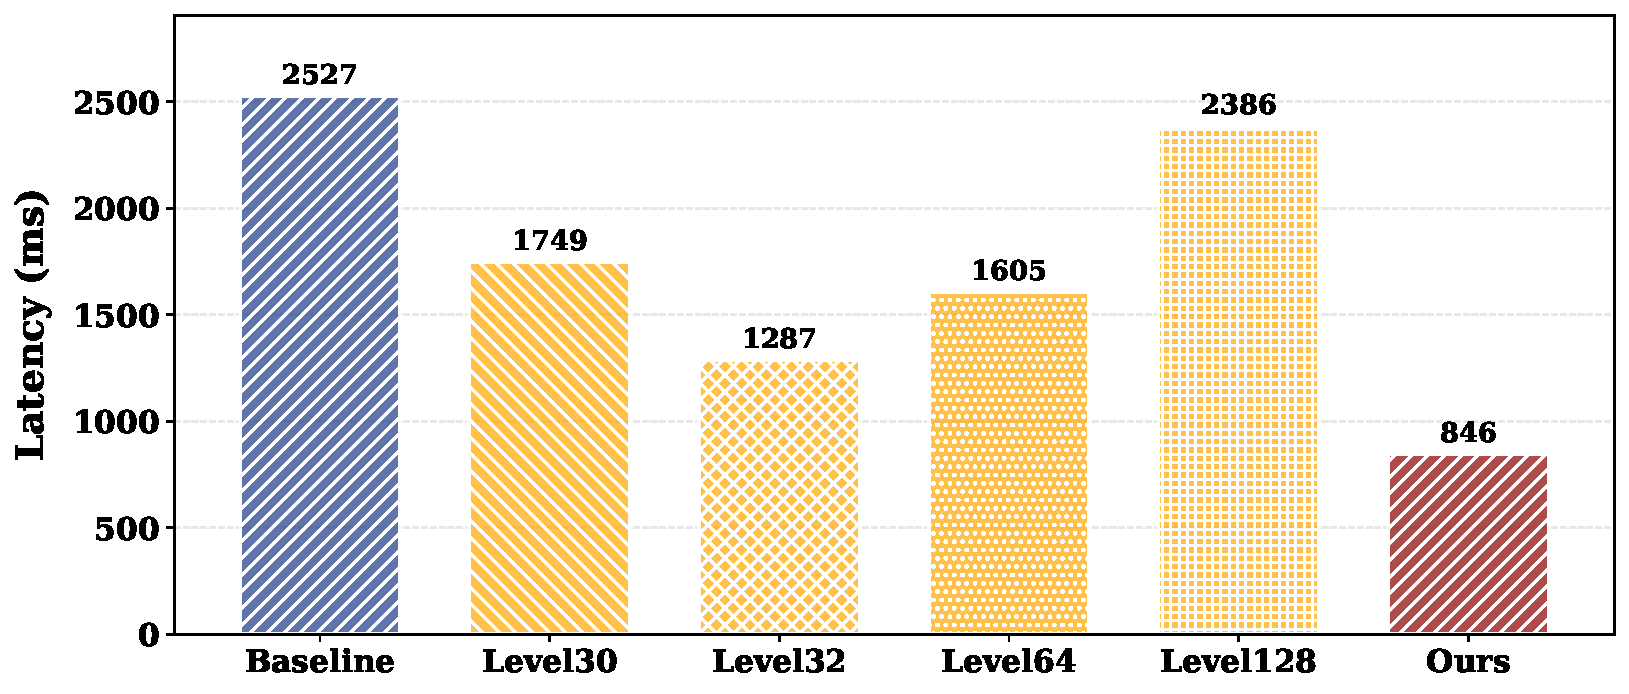
\includegraphics[width=0.98\linewidth]{figure/admission_levels_comparison.pdf}
    \caption{End-to-end latency under fixed vs adaptive admission control for Qwen3-32B (Batch 256, TP 2, 2 GPUs).}
    \label{fig:e2ecache}
    % \vvspace{}
\end{figure}